% Options for packages loaded elsewhere
\PassOptionsToPackage{unicode}{hyperref}
\PassOptionsToPackage{hyphens}{url}
%
\documentclass[
]{article}
\usepackage{amsmath,amssymb}
\usepackage{iftex}
\ifPDFTeX
  \usepackage[T1]{fontenc}
  \usepackage[utf8]{inputenc}
  \usepackage{textcomp} % provide euro and other symbols
\else % if luatex or xetex
  \usepackage{unicode-math} % this also loads fontspec
  \defaultfontfeatures{Scale=MatchLowercase}
  \defaultfontfeatures[\rmfamily]{Ligatures=TeX,Scale=1}
\fi
\usepackage{lmodern}
\ifPDFTeX\else
  % xetex/luatex font selection
\fi
% Use upquote if available, for straight quotes in verbatim environments
\IfFileExists{upquote.sty}{\usepackage{upquote}}{}
\IfFileExists{microtype.sty}{% use microtype if available
  \usepackage[]{microtype}
  \UseMicrotypeSet[protrusion]{basicmath} % disable protrusion for tt fonts
}{}
\makeatletter
\@ifundefined{KOMAClassName}{% if non-KOMA class
  \IfFileExists{parskip.sty}{%
    \usepackage{parskip}
  }{% else
    \setlength{\parindent}{0pt}
    \setlength{\parskip}{6pt plus 2pt minus 1pt}}
}{% if KOMA class
  \KOMAoptions{parskip=half}}
\makeatother
\usepackage{xcolor}
\usepackage[margin=1in]{geometry}
\usepackage{color}
\usepackage{fancyvrb}
\newcommand{\VerbBar}{|}
\newcommand{\VERB}{\Verb[commandchars=\\\{\}]}
\DefineVerbatimEnvironment{Highlighting}{Verbatim}{commandchars=\\\{\}}
% Add ',fontsize=\small' for more characters per line
\usepackage{framed}
\definecolor{shadecolor}{RGB}{248,248,248}
\newenvironment{Shaded}{\begin{snugshade}}{\end{snugshade}}
\newcommand{\AlertTok}[1]{\textcolor[rgb]{0.94,0.16,0.16}{#1}}
\newcommand{\AnnotationTok}[1]{\textcolor[rgb]{0.56,0.35,0.01}{\textbf{\textit{#1}}}}
\newcommand{\AttributeTok}[1]{\textcolor[rgb]{0.13,0.29,0.53}{#1}}
\newcommand{\BaseNTok}[1]{\textcolor[rgb]{0.00,0.00,0.81}{#1}}
\newcommand{\BuiltInTok}[1]{#1}
\newcommand{\CharTok}[1]{\textcolor[rgb]{0.31,0.60,0.02}{#1}}
\newcommand{\CommentTok}[1]{\textcolor[rgb]{0.56,0.35,0.01}{\textit{#1}}}
\newcommand{\CommentVarTok}[1]{\textcolor[rgb]{0.56,0.35,0.01}{\textbf{\textit{#1}}}}
\newcommand{\ConstantTok}[1]{\textcolor[rgb]{0.56,0.35,0.01}{#1}}
\newcommand{\ControlFlowTok}[1]{\textcolor[rgb]{0.13,0.29,0.53}{\textbf{#1}}}
\newcommand{\DataTypeTok}[1]{\textcolor[rgb]{0.13,0.29,0.53}{#1}}
\newcommand{\DecValTok}[1]{\textcolor[rgb]{0.00,0.00,0.81}{#1}}
\newcommand{\DocumentationTok}[1]{\textcolor[rgb]{0.56,0.35,0.01}{\textbf{\textit{#1}}}}
\newcommand{\ErrorTok}[1]{\textcolor[rgb]{0.64,0.00,0.00}{\textbf{#1}}}
\newcommand{\ExtensionTok}[1]{#1}
\newcommand{\FloatTok}[1]{\textcolor[rgb]{0.00,0.00,0.81}{#1}}
\newcommand{\FunctionTok}[1]{\textcolor[rgb]{0.13,0.29,0.53}{\textbf{#1}}}
\newcommand{\ImportTok}[1]{#1}
\newcommand{\InformationTok}[1]{\textcolor[rgb]{0.56,0.35,0.01}{\textbf{\textit{#1}}}}
\newcommand{\KeywordTok}[1]{\textcolor[rgb]{0.13,0.29,0.53}{\textbf{#1}}}
\newcommand{\NormalTok}[1]{#1}
\newcommand{\OperatorTok}[1]{\textcolor[rgb]{0.81,0.36,0.00}{\textbf{#1}}}
\newcommand{\OtherTok}[1]{\textcolor[rgb]{0.56,0.35,0.01}{#1}}
\newcommand{\PreprocessorTok}[1]{\textcolor[rgb]{0.56,0.35,0.01}{\textit{#1}}}
\newcommand{\RegionMarkerTok}[1]{#1}
\newcommand{\SpecialCharTok}[1]{\textcolor[rgb]{0.81,0.36,0.00}{\textbf{#1}}}
\newcommand{\SpecialStringTok}[1]{\textcolor[rgb]{0.31,0.60,0.02}{#1}}
\newcommand{\StringTok}[1]{\textcolor[rgb]{0.31,0.60,0.02}{#1}}
\newcommand{\VariableTok}[1]{\textcolor[rgb]{0.00,0.00,0.00}{#1}}
\newcommand{\VerbatimStringTok}[1]{\textcolor[rgb]{0.31,0.60,0.02}{#1}}
\newcommand{\WarningTok}[1]{\textcolor[rgb]{0.56,0.35,0.01}{\textbf{\textit{#1}}}}
\usepackage{graphicx}
\makeatletter
\def\maxwidth{\ifdim\Gin@nat@width>\linewidth\linewidth\else\Gin@nat@width\fi}
\def\maxheight{\ifdim\Gin@nat@height>\textheight\textheight\else\Gin@nat@height\fi}
\makeatother
% Scale images if necessary, so that they will not overflow the page
% margins by default, and it is still possible to overwrite the defaults
% using explicit options in \includegraphics[width, height, ...]{}
\setkeys{Gin}{width=\maxwidth,height=\maxheight,keepaspectratio}
% Set default figure placement to htbp
\makeatletter
\def\fps@figure{htbp}
\makeatother
\setlength{\emergencystretch}{3em} % prevent overfull lines
\providecommand{\tightlist}{%
  \setlength{\itemsep}{0pt}\setlength{\parskip}{0pt}}
\setcounter{secnumdepth}{-\maxdimen} % remove section numbering
\usepackage{booktabs}
\usepackage{longtable}
\usepackage{array}
\usepackage{multirow}
\usepackage{wrapfig}
\usepackage{float}
\usepackage{colortbl}
\usepackage{pdflscape}
\usepackage{tabu}
\usepackage{threeparttable}
\usepackage{threeparttablex}
\usepackage[normalem]{ulem}
\usepackage{makecell}
\usepackage{xcolor}
\ifLuaTeX
  \usepackage{selnolig}  % disable illegal ligatures
\fi
\IfFileExists{bookmark.sty}{\usepackage{bookmark}}{\usepackage{hyperref}}
\IfFileExists{xurl.sty}{\usepackage{xurl}}{} % add URL line breaks if available
\urlstyle{same}
\hypersetup{
  pdftitle={Taller\_2},
  pdfauthor={John Esteban},
  hidelinks,
  pdfcreator={LaTeX via pandoc}}

\title{Taller\_2}
\author{John Esteban}
\date{2024-03-25}

\begin{document}
\maketitle

\begin{verbatim}
## Loading required package: usethis
\end{verbatim}

\begin{verbatim}
## 
## Attaching package: 'dplyr'
\end{verbatim}

\begin{verbatim}
## The following object is masked from 'package:kableExtra':
## 
##     group_rows
\end{verbatim}

\begin{verbatim}
## The following object is masked from 'package:gridExtra':
## 
##     combine
\end{verbatim}

\begin{verbatim}
## The following objects are masked from 'package:stats':
## 
##     filter, lag
\end{verbatim}

\begin{verbatim}
## The following objects are masked from 'package:base':
## 
##     intersect, setdiff, setequal, union
\end{verbatim}

\begin{verbatim}
## i SHA-1 hash of file is "08930743b60b5cdcfadeb8abaa79e488be87522f"
## -- Attaching core tidyverse packages ------------------------ tidyverse 2.0.0 --
## v forcats   1.0.0     v readr     2.1.5
## v ggplot2   3.4.4     v stringr   1.5.1
## v lubridate 1.9.3     v tibble    3.2.1
## v purrr     1.0.2     v tidyr     1.3.1
## -- Conflicts ------------------------------------------ tidyverse_conflicts() --
## x dplyr::combine()        masks gridExtra::combine()
## x dplyr::filter()         masks stats::filter()
## x dplyr::group_rows()     masks kableExtra::group_rows()
## x readr::guess_encoding() masks rvest::guess_encoding()
## x dplyr::lag()            masks stats::lag()
## i Use the conflicted package (<http://conflicted.r-lib.org/>) to force all conflicts to become errors
## i SHA-1 hash of file is "3ff8c4f235a8505f47a4ebea967cbede1a557c4c"
\end{verbatim}

\hypertarget{introduccion}{%
\section{Introduccion}\label{introduccion}}

La pobreza es uno de los temas centrales de investigación en la economía
del bienestar y en las agendas políticas de todos los gobiernos,
especialmente en los países en vías de desarrollo. Sin embargo, no hay
un consenso en su definición y en su forma de ser medida. A pesar de
esto, se puede entender que ser pobre es no disponer de los recursos
para obtener los medios mínimos de subsistencia, una definición general.
El Banco Mundial define la pobreza como incapacidades para llevar una
vida plena, desagregándolo en buena alimentación, calidad de la
vivienda, buena salud, buena educación y tener un trabajo digno. También
tenemos la definición de uno de los economistas que más influencia tiene
en el estudio de la pobreza, Amartya Sen.~Con la teoría de las
capacidades, este autor dice que la pobreza no es simplemente la falta
de ingreso, sino la falta de capacidades básicas y la libertad para
obtenerlo, definición muy parecida a la propuesta del Banco Mundial. En
resumen, los avances del estudio teórico de la pobreza han reposado en
que es un fenómeno multidimensional y no solamente carencia de ingresos.

De la misma forma que las definiciones, la forma de medir la pobreza es
variada, donde se tiene en cuenta la multidimensionalidad de la pobreza
que tanto se menciona en la etapa de definición. En primer lugar, se
tiene el NBI (Necesidades Básicas Insatisfechas) que señala la
insuficiencia que tiene un hogar en una de las siguientes necesidades
básicas: Vivienda con Materiales adecuados, servicios públicos de
acueducto y alcantarillado, nivel bajo de hacinamiento, bajo grado de
dependencia. También se encuentra el método de la línea de pobreza, que
calcula el costo de una canasta básica de bienes y servicios, luego
calcula los ingresos del hogar y se compara con esta línea, si no
alcanza este mínimo entonces se considera un hogar pobre. Por último,
también se trabaja con el Índice de Condiciones de vida, que comprende
variables que miden la calidad de la vivienda, el capital humano actual
y potencial, el acceso a la calidad de los servicios y las condiciones
del hogar. En este trabajo se va a trabajar con el indicador de línea de
pobreza.

El objetivo de este artículo es encontrar los determinantes económicos y
sociales que más inciden en clasificar a una persona como pobre o no
pobre a través de la medida de línea de pobreza. Para esto se utilizan
los datos del DANE que vienen de la Misión de Empalme de las Series de
Empleo, Pobreza y Desigualdad. En esta base de datos se encuentra a
nivel de hogar y de personas y recoge toda la información sobre las
condiciones de empleo de las personas, además de todas las
características socioeconómicas generales y que son importantes para
determinar la pobreza de un hogar. Por tanto, con estas variables se
puede estimar en términos de probabilidades las características de la
población menos favorecida.

El estudio de los determinantes de la pobreza es importante porque
muestra los temas en los que es necesario focalizar las políticas
públicas. En Colombia se han realizado varios estudios que buscan
encontrar los determinantes de la pobreza con datos de tipo transversal.
Nunes \& Ramírez (2002) utilizan un modelo de respuesta cualitativa para
encontrar las características socioeconómicas de los hogares más pobres
a través de la estimación de probabilidades. Estos autores encuentran
que el nivel educativo, la cantidad de los miembros del hogar, la tasa
de ocupación y la ubicación del hogar son variables que afectan la
probabilidad de ser o no hogares pobres.

En la misma dirección, Chaves (2010) encuentra con un modelo logit que
la educación del jefe de hogar, la posesión de activos, el tamaño del
hogar, el tipo de vivienda y el género del jefe de hogar son
determinantes de que este se encuentre o no en situación de pobreza. De
esta forma, la mayoría de los estudios de los determinantes de la
pobreza tienen una forma similar de trabajar, se establecen las
variables de control, se crea la variable de respuesta binaria a través
de la línea de pobreza y se procede con la estimación de los parámetros
con modelos probit o logit (Nunes \& Ramírez, 2002), (Nunes, Ramírez,
Cuesta, 2005), (Chaves, 2010), (Marrugo et al., 2015).

Un factor común que utilizan todos los estudios es trabajar y estimar la
pobreza de un hogar a través de las condiciones del jefe de hogar, esto
debido a que es el responsable sobre todo económico de todos los
integrantes. Por esta razón, es importante estudiar la posición del jefe
de hogar en el mercado laboral, ya que muestra la capacidad de los
ingresos y calidad de vida. Investigar sobre su posición en el mercado y
si trabaja en condiciones de informalidad puede ser un determinante de
la condición de pobreza. Esto debido a que trabajar en condiciones de
informalidad, por sus características precarias y bajos salarios, puede
explicar la pobreza en un hogar (Torres et al., 2022). También la edad
del jefe de hogar puede servir como determinante de la pobreza porque,
desde la teoría, se considera que hay edades donde es tiene más
incidencia el desempleo como en la población joven y más adulta (Klose,
2012).

\hypertarget{datos}{%
\section{Datos}\label{datos}}

\hypertarget{seleccion-de-los-datos}{%
\subsection{Seleccion de los datos}\label{seleccion-de-los-datos}}

La seleccion de las variables se hacen tomando como referencia los
estudios analizados para este proceso y todo se trabaja a nivel de hogar
como lo recomienda Chaves(2010), (Torres, et al,2022), (Klose,2012)

\begin{itemize}
\tightlist
\item
  p6050: Si es jefe de hogar
\item
  p620: Sexo del jefe de hogar
\item
  p6100: Tipo de regimen
\item
  p6210: Educacion
\item
  p6240: Empleado
\item
  p6430: Posicion laboral del jefe de hogar
\item
  Personas por habitacion
\item
  Tipo de vivienda: propia o no
\item
  Edad del jefe de hogar
\item
  Zona: Rural o Urbana
\item
  Tipo de trabajo
\end{itemize}

\hypertarget{limpieza-de-los-datos.}{%
\subsection{Limpieza de los datos.}\label{limpieza-de-los-datos.}}

Todo el analisis exploratorio de datos y la modelación se hace para las
personas que han reportado que son jefes de hogar, por esto la limpieza
mas importante es crear la variable jefe, que establece que si es jefe
de hogar tiene el valor de 1 y 0 en los otros caso, por esto al momento
de traer las variables del nivel de personas al de hogar se hace tomando
como referencia si es jefe de hogar,

\begin{Shaded}
\begin{Highlighting}[]
\NormalTok{train\_personas}\SpecialCharTok{$}\NormalTok{jefe}\OtherTok{\textless{}{-}}\FunctionTok{ifelse}\NormalTok{(}\AttributeTok{test =}\NormalTok{ train\_personas}\SpecialCharTok{$}\NormalTok{P6050}\SpecialCharTok{==}\DecValTok{1}\NormalTok{,}\DecValTok{1}\NormalTok{,}\DecValTok{0}\NormalTok{)}
\NormalTok{test\_personas}\SpecialCharTok{$}\NormalTok{jefe}\OtherTok{\textless{}{-}}\FunctionTok{ifelse}\NormalTok{(}\AttributeTok{test =}\NormalTok{ test\_personas}\SpecialCharTok{$}\NormalTok{P6050}\SpecialCharTok{==}\DecValTok{1}\NormalTok{,}\DecValTok{1}\NormalTok{,}\DecValTok{0}\NormalTok{)}
\end{Highlighting}
\end{Shaded}

Para automatizar el proceso de traer las caracteristicas que pueden
explicar la pobreza monetaria de un hogar se crea la función crear\_,
que tiene el siguiente funcionamiento. Primero se guarda la función
segun seal nombre de la variable a traer, esta funcion recibe como
parametro la base de datos sobre la cual se va a construir la variable,
el primer filtro que se aplica es que en la base de datos de personas
debe estar filtrada solo para los jefes de hogar, del dataframe se toma
la variable de interes junto con el identificador unico de personas que
crea la base de datos y por ultimo se crea el join con la base de datos
de hogares por medio de este identificador. La función llamada traer
variable garantiza que no se repitan los id y que tenenmos registros
unicos en toda la muestra.

\begin{Shaded}
\begin{Highlighting}[]
\NormalTok{crear\_sexo\_jefe}\OtherTok{\textless{}{-}}\ControlFlowTok{function}\NormalTok{(df)\{}
\NormalTok{  aux}\OtherTok{\textless{}{-}}\NormalTok{df }\SpecialCharTok{\%\textgreater{}\%} \FunctionTok{filter}\NormalTok{(jefe}\SpecialCharTok{==}\DecValTok{1}\NormalTok{)}
\NormalTok{  aux2}\OtherTok{\textless{}{-}}\FunctionTok{data.frame}\NormalTok{(}\AttributeTok{sexo\_jefe=}\NormalTok{aux}\SpecialCharTok{$}\NormalTok{P6020,}\AttributeTok{id=}\NormalTok{aux}\SpecialCharTok{$}\NormalTok{id)}
\NormalTok{  df}\OtherTok{\textless{}{-}}\FunctionTok{left\_join}\NormalTok{(df,aux2,}\AttributeTok{by=}\StringTok{"id"}\NormalTok{)}
  \FunctionTok{return}\NormalTok{(df)}
\NormalTok{\}}
\NormalTok{train\_personas}\OtherTok{\textless{}{-}}\FunctionTok{crear\_sexo\_jefe}\NormalTok{(train\_personas)}
\NormalTok{train\_hogares}\OtherTok{\textless{}{-}}\FunctionTok{traer\_variable}\NormalTok{(train\_hogares,train\_personas,}\StringTok{"sexo\_jefe"}\NormalTok{)}
\NormalTok{train\_hogares}\SpecialCharTok{$}\NormalTok{sexo\_jefe}\OtherTok{\textless{}{-}}\FunctionTok{as.factor}\NormalTok{(train\_hogares}\SpecialCharTok{$}\NormalTok{sexo\_jefe)}

\NormalTok{test\_personas}\OtherTok{\textless{}{-}}\FunctionTok{crear\_sexo\_jefe}\NormalTok{(test\_personas)}
\NormalTok{test\_hogares}\OtherTok{\textless{}{-}}\FunctionTok{traer\_variable}\NormalTok{(test\_hogares,test\_personas,}\StringTok{"sexo\_jefe"}\NormalTok{)}
\NormalTok{test\_hogares}\SpecialCharTok{$}\NormalTok{sexo\_jefe}\OtherTok{\textless{}{-}}\FunctionTok{as.factor}\NormalTok{(test\_hogares}\SpecialCharTok{$}\NormalTok{sexo\_jefe)}
\end{Highlighting}
\end{Shaded}

Este proceso se hace para cada una de las variables , en este dosumento
solo se presenta el caso para el sexo del jefe del hogar, en el script
Creación de variables de interes esta el proceso para cada una de las
variables.

Este proceso se hace para las siguientes variables:

\includegraphics{Taller_2_files/figure-latex/unnamed-chunk-5-1.pdf}

\hypertarget{analisis-exploratorio-de-los-datos}{%
\subsection{Analisis exploratorio de los
datos}\label{analisis-exploratorio-de-los-datos}}

El analisis exploratorio se datos se divide en dos partes: Analisis
univariado y analisis multivariado de datos. En el analisis univariado
el proposito es analizar como se distribuyen de forma individual las
variables que vamos a utilizar en el proceso de modelacion. Luego con el
analisis multivariado nuestro objetivo es ver como se relacionan las
variable independientes con el ingreso de los hogares.

\hypertarget{analisis-univariado}{%
\subsubsection{Analisis univariado}\label{analisis-univariado}}

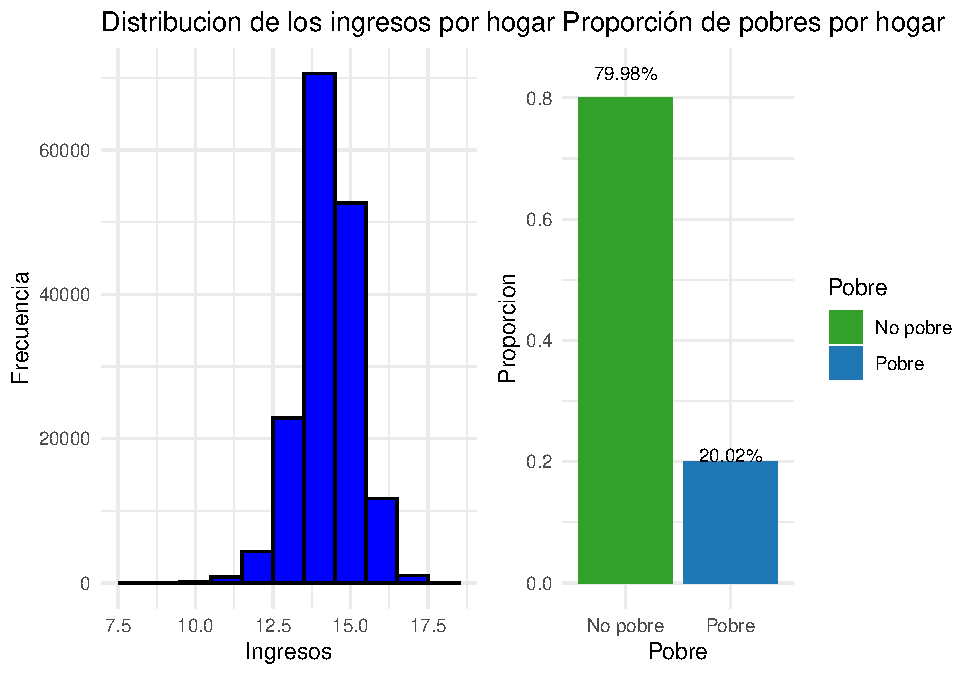
\includegraphics{Taller_2_files/figure-latex/unnamed-chunk-6-1.pdf}

Estas son las dos variables objetivo que se van a explicar en este
informe. En la primera gráfica se presentan los ingresos agregados del
hogar, que se utilizan para determinar si un hogar es pobre utilizando
la línea de pobreza, mientras que la variable `Pobre' está categorizada
como 0 cuando el hogar no es pobre y 1 cuando lo es. Los datos muestran
que aproximadamente el 80\% de los hogares no están en condición de
pobreza, lo que implica un desafío en términos del proceso de modelado
debido a que hay un claro desbalance de clases.

\hypertarget{variables-explicativas}{%
\subsubsection{Variables explicativas}\label{variables-explicativas}}

\includegraphics{Taller_2_files/figure-latex/unnamed-chunk-7-1.pdf}

En este caso, observamos que la representación de jefes de hogar
masculinos es ligeramente mayor que la de las mujeres que encabezan el
hogar. Según la literatura económica, cuando la mujer es la jefa de
hogar, existe un mayor riesgo de pobreza en el hogar. Esta situación
puede atribuirse a diversos factores, como la brecha salarial de género
y la responsabilidad desproporcionada de cuidado y trabajo doméstico no
remunerado.

Respecto a los jefes de hogar afiliados al régimen subsidiado,
representan aproximadamente el 42\% del total. Esta variable es crucial
de analizar, ya que el acceso a este mecanismo por parte de los
colombianos para obtener servicios cuando no tienen capacidad de pago,
sirve como una medida indirecta de la condición de pobreza de un hogar.

\includegraphics{Taller_2_files/figure-latex/unnamed-chunk-8-1.pdf}

Para revisar la educación de los jefes de hogar, primero se filtran
aquellos que no saben o no responden, y se calcula la proporción con
respecto al total de personas que reportaron su nivel educativo. En este
análisis, observamos que la mayoría de los jefes de hogar tienen al
menos aprobada la educación básica secundaria. Esta variable es una de
las más importantes para predecir el nivel de ingresos de un hogar. Como
se mencionó en la introducción de este informe, a medida que el jefe de
hogar obtiene un mayor nivel de educación formal, la probabilidad de ser
pobre disminuye, ya que una mayor educación se traduce en mayores
niveles de ingresos. Sin embargo, es preocupante la gran cantidad de
personas que no reportan su último nivel educativo alcanzado.

El estado de empleo es fundamental para determinar si un hogar está en
condición de pobreza. Esto se explica porque si el jefe de hogar está
desempleado, significa que el hogar no está percibiendo ingresos por
parte de la persona encargada del sustento familiar, lo cual aumenta la
probabilidad de ser pobre. En este caso, observamos que aproximadamente
el 37\% de los jefes de hogar no están empleados, una cifra considerable
que puede explicar la situación del hogar.

\includegraphics{Taller_2_files/figure-latex/unnamed-chunk-9-1.pdf}

La posición del jefe de hogar en el empleo es importante para determinar
si el hogar corre riesgo de estar en situación de pobreza. Se espera que
los jefes de hogar que trabajen sin remuneración tengan un mayor riesgo
de pobreza. Sin embargo, en nuestro análisis no se observa que esta sea
la situación predominante, ya que al combinar estas dos categorías
apenas llegan al 1\%.

Tener casa propia, en principio, puede ayudar a explicar la situación de
pobreza del hogar. Esto se debe a que contar con una vivienda propia
permite disponer de una mayor cantidad de ingresos que pueden destinarse
a cubrir otras necesidades. La propiedad de una casa se considera una
inversión y un seguro en momentos de dificultades económicas. Se supone
que las personas que no tienen casa propia podrían ser más vulnerables
relativamente a ser pobres. En nuestra muestra, observamos que la
mayoría de los jefes de hogar no cuentan con vivienda propia y deben
pagar arriendo por su alojamiento. Es fundamental profundizar en esta
información para comprender mejor la dinámica de la pobreza en los
hogares.

\includegraphics{Taller_2_files/figure-latex/unnamed-chunk-10-1.pdf}

El número de personas por habitación también se considera importante
para predecir la pobreza, ya que se espera que a mayor número de
personas por habitación, exista un hacinamiento que aumente el riesgo de
pobreza. En nuestro análisis, la mayoría de los datos se concentran en 2
personas por habitación, lo cual es una situación normal.

Es fundamental incorporar la edad del jefe del hogar en nuestro
análisis, ya que está intrínsecamente ligada a la teoría del ciclo de
vida en economía, la cual postula que las personas atraviesan diferentes
etapas en su vida, cada una con características económicas específicas
que pueden influir en su vulnerabilidad a la pobreza.

En el contexto colombiano, esta teoría cobra especial relevancia, ya que
tanto los jóvenes como los ancianos son considerados grupos de población
vulnerables. Por un lado, los jóvenes tienden a enfrentar mayores
dificultades económicas debido a su entrada reciente al mercado laboral
y su menor experiencia, lo que puede traducirse en ingresos más bajos y
una mayor vulnerabilidad financiera. Este fenómeno se ve exacerbado por
las altas tasas de desempleo que suelen afectar a este grupo
demográfico. Por lo tanto, es plausible suponer que los jefes de hogar
más jóvenes enfrenten desafíos adicionales para alcanzar la estabilidad
financiera, lo que podría aumentar su probabilidad de experimentar
situaciones de pobreza.

Por otro lado, la teoría del ciclo de vida también reconoce que los
ancianos, especialmente después de su retiro, pueden enfrentar
dificultades económicas debido a ingresos fijos y limitados, como
pensiones o jubilaciones, que pueden no ser suficientes para cubrir
todas sus necesidades. A pesar de haber contribuido al mercado laboral
durante años, las limitaciones en los ingresos de jubilación pueden
dejar a los ancianos en una situación económica precaria, lo que aumenta
la probabilidad de que los hogares encabezados por personas mayores
estén en situación de pobreza.

Si bien en nuestra muestra de datos observamos una distribución uniforme
de las edades de los jefes de hogar, la teoría del ciclo de vida nos
permite anticipar que los hogares liderados por personas más jóvenes y
más mayores podrían enfrentar mayores dificultades económicas, cada uno
por razones asociadas a su etapa de vida.

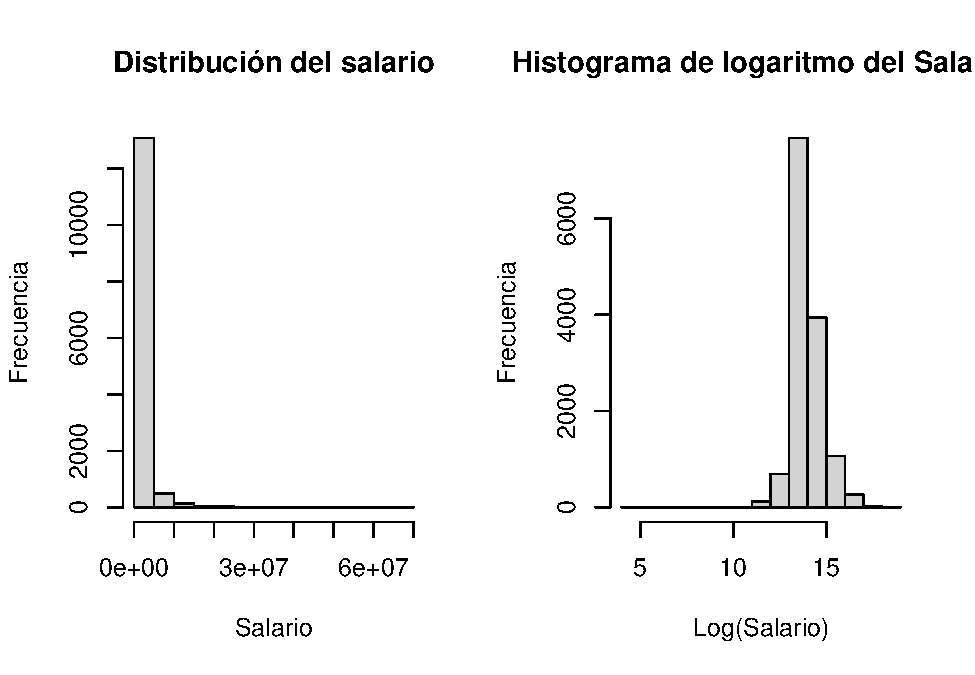
\includegraphics{Taller_2_files/figure-latex/unnamed-chunk-11-1.pdf}

La distinción entre el tipo de empleo a través de la informalidad
laboral es un factor crucial para determinar las condiciones de pobreza
de un hogar. El trabajo informal se caracteriza por salarios bajos y
condiciones laborales precarias, lo que puede aumentar
significativamente el riesgo de pobreza para quienes se desempeñan en
este sector. En nuestros datos, observamos que aproximadamente el 47\%
de las personas trabajan en condiciones de informalidad, una cifra que
concuerda con los datos nacionales y subraya la magnitud del desafío que
representa la informalidad laboral en términos de pobreza.

Además, la ubicación geográfica del hogar también desempeña un papel
crucial, ya que las viviendas ubicadas en áreas más alejadas del centro
económico suelen considerarse más vulnerables. Esta disparidad se
explica en parte por la teoría del centro-periferia, que destaca las
diferencias en el desarrollo económico entre las áreas urbanas centrales
y las regiones periféricas. En el contexto urbano, el centro se
caracteriza por un mayor desarrollo económico e industrial, mientras que
las áreas rurales tienden a tener un menor desarrollo, con actividades
económicas centradas en la agricultura y la extracción de recursos, que
generalmente se asocian con salarios más bajos. Aunque en nuestra
muestra hay una representación limitada del área rural, este análisis
nos brinda una aproximación útil para evaluar la probabilidad de pobreza
en función de la ubicación del hogar y su relación con la teoría del
centro-periferia.

\includegraphics{Taller_2_files/figure-latex/unnamed-chunk-12-1.pdf}

En la gráfica anterior, se observan las variables seleccionadas en
relación con el logaritmo de los ingresos del hogar. Este enfoque se
utiliza para normalizar los datos y facilitar la comparación entre las
variables de interés. En términos generales, se puede apreciar que las
personas afiliadas al régimen subsidiado tienen ingresos ligeramente
inferiores en comparación con aquellos que son cotizantes. Del mismo
modo, se evidencia que las personas desempleadas tienden a tener
ingresos menores en el hogar. En cuanto al sexo del jefe de hogar, las
diferencias en los ingresos no son tan marcadas. Sin embargo, se
observan diferencias significativas en los ingresos agregados según el
nivel educativo del jefe de hogar y su posición laboral.

Además, se aprecia que a medida que aumenta el número de personas por
habitación, la media de ingresos del hogar tiende a disminuir, lo cual
coincide con lo reportado en la literatura. Respecto a las variables
tipo\_casa y edad\_jefe\_joven, los resultados son coherentes con lo
esperado, ya que los jefes de hogar que poseen vivienda propia y son
adultos suelen tener mayores ingresos, lo que reduce la probabilidad de
estar en situación de pobreza.

El tema de la informalidad laboral también muestra diferencias
significativas en los ingresos de las personas. En general, aquellos que
trabajan en condiciones de informalidad tienen ingresos más bajos, lo
que aumenta su vulnerabilidad económica y, por ende, la probabilidad de
estar en situación de pobreza.

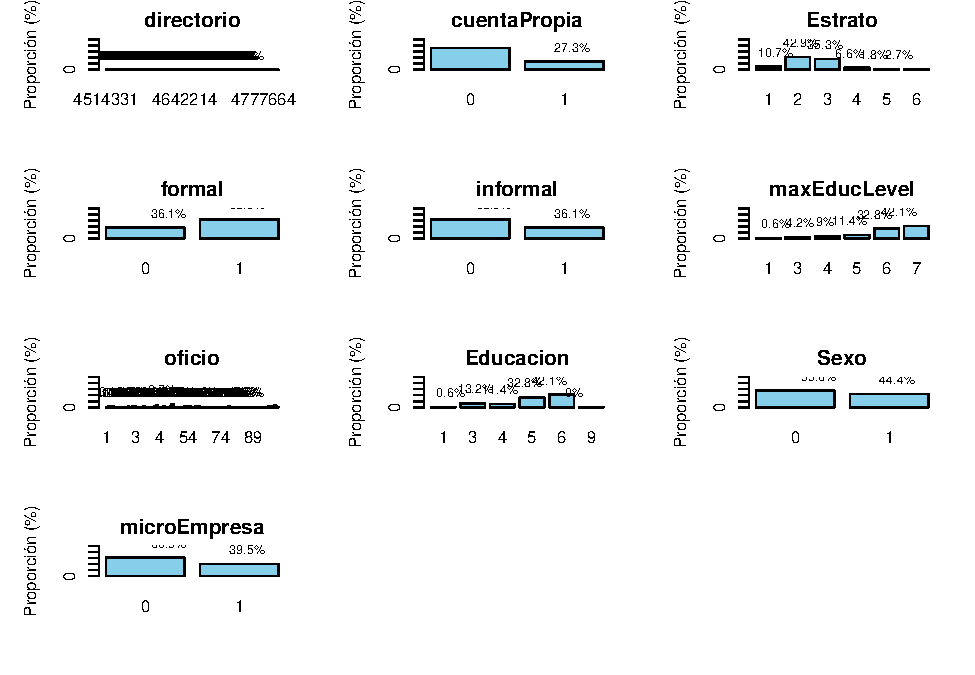
\includegraphics{Taller_2_files/figure-latex/unnamed-chunk-13-1.pdf}

Cuando se analiza en relación con la variable de pobreza, se observa un
patrón muy similar al analizar los ingresos del hogar. Sin embargo, se
destaca que la tenencia de vivienda propia marca una diferencia más
significativa que cuando se analiza únicamente por medio de los
ingresos. Esto sugiere que la posesión de vivienda propia puede ser un
factor más determinante en la reducción de la probabilidad de pobreza,
independientemente de los niveles de ingresos del hogar.

\hypertarget{estimacion-de-los-modelos}{%
\section{Estimacion de los modelos}\label{estimacion-de-los-modelos}}

\hypertarget{conclusiones}{%
\section{Conclusiones}\label{conclusiones}}

\end{document}
